
% halfedge data structure has proven successful.

3D polygon surface mesh data structures based on the concept of
halfedges~\cite{k-ugpdd-99} have been very successful for the design
of general algorithms on meshes. (do we mention it is a standard
building block used for research or industry-strength softwares? we
need adding references if so).

% focus on algorithms, not on data structures.

Although making a preliminary version of a halfedge-based mesh data
structure is as a fairly simple task and is often proposed as a
programming exercice, the time has come where we should not write our
own mesh data structure from scratch anymore. 

I list a bunch of reasons here, and let you reduce/extend them.

Not reinventing the wheel, hence learning how to integrate an existing
tool makes a real added value. Implementing a mesh data structure from
scratch makes a zero added value to your algorithms.

Using a bug-free mesh data structure eases the implementation and
helps focusing on the end-goal, i.e. the algorithms rather than
debugging the underlying data structure.

Using a robust and optimized data structure allows to obtain fast and
robust results. The time has gone where toy examples were sufficient
to illustrate research results (ref. repository of big models
standardly used in graphics). The data structure must scale linearly
with the mesh complexity.

Choose a data structure that adopts the generic programming paradigm.
Generic programming saves time and effort and allows the reuse of
existing data structures and algorithms. (there are many other
argument for generic programming that we should list here - long error
messages are not for example).

Your algorithms on meshes usually needs more than a mesh data
structure, e.g. basic geometric entities such as points, vectors,
planes and simple operations acting upon them (distance,
intersections, orientation).

What you need is a library, flexible enough to let you elaborate your
own algorithm on meshes while reusing all basic geometric computing
components.

Choose one library that has emerged as a standard in a community.
Such kind of libraries usually offer support and discussion lists
(extremely helpful before siggraph deadlines).

CGAL and the demo programs accompanying this tutorial offer a viable
solution that we present here. (we have to compare us with the
OpenMesh project within OpenSG).

% intended audience

The intended audience are researchers, developers or students in the
graphics community developing algorithms around meshes.

% the solution

The solution contains a flexible, powerful and efficient mesh data
structure, examples of algorithms on meshes, such as subdivision
surfaces, (self-) intersection tests, estimation of curvatures,
convenient file IO with Wavefront OBJ and OFF formats, an interactive
visualization program for inspection, debugging, experimenting, and
support for preparing pictures for publications.

% teaser 
\begin{figure}[htb]
    \centering{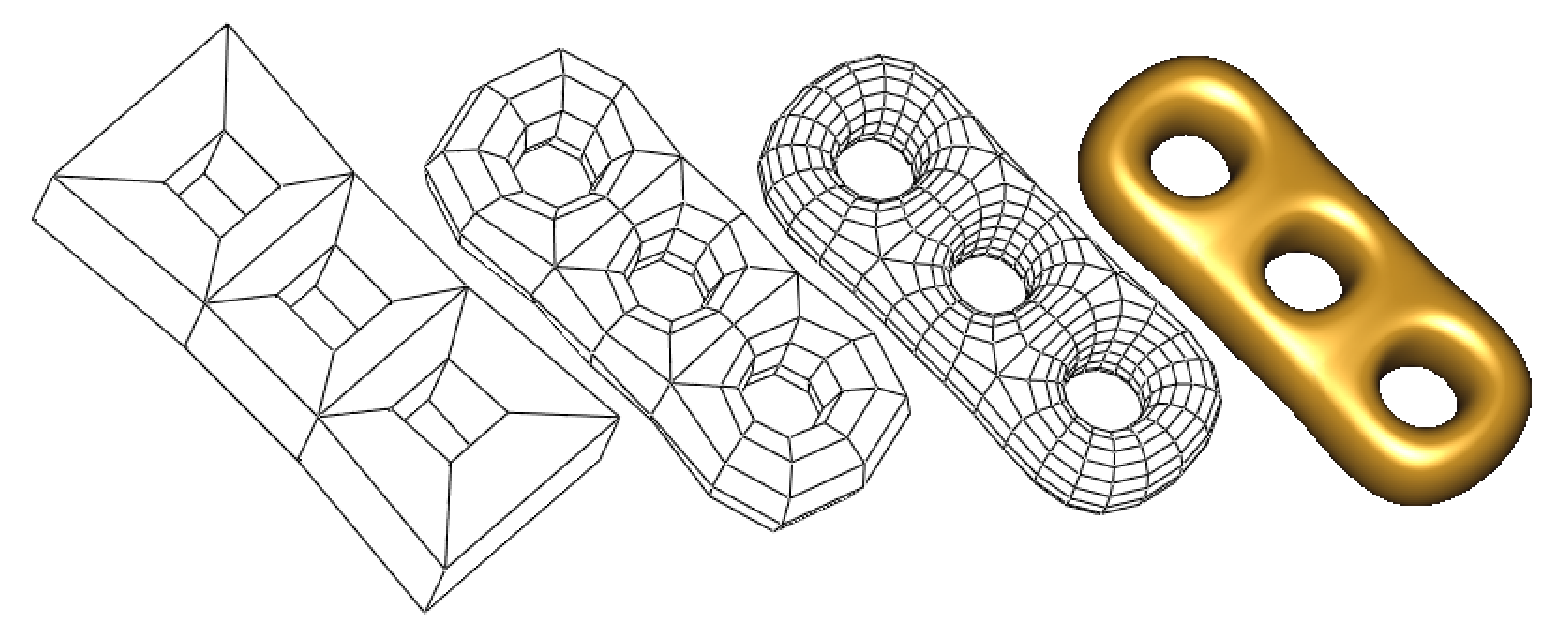
\includegraphics[width=12.0cm]{figs/teaser}}
    \caption{Demo application running on Windows. A polygon mesh is 
             subdivided using the quad-triangle subdivision 
             scheme~\cite{sl-qts-02}.}
    \label{fig:teaser}
\end{figure}



% open

Open source and contributions are welcome. 



% remainder

Section 2 describes how to declare a polyhedron, read a polygon mesh
from a file, and iterate over all facets for rendering. Example is
shown to enrich a polyhedron with extended primitives (normals,
colors, curvature tensors).

Section 3 illustrates how to write subdivision algorithms for meshes
(since they act on both connectivity and geometry, it is perfect for
our training purpose). Three approaches are shown. First one is sqrt3
subdivision using Euler operators. Second one uses the incremental
builder (originally designed for file IO) with a control mesh as
input. Third one offers a generic design for writing subdivision
algorithms.



% Andy

%program 1: rendering and file io of a default polyhedron 
%   context: a skeleton of a polyhedron program: declaration,
%initialization (inc. builder) and the rendering (iteration on facet and
%circulation of the factes)

%program 2: enriched polyhedron in program 1
%   context: extend a polyhedron: trait, item. hds? Use of the extended
%primitives.

%program 3: subdivision 1 (sqrt3)
%   context: refinement operators. Halfedge trversal (prev(), etc...) and
%circulators. Effect of connectivity edit on iterator and circulator.
%Maintain the correspondence after refinement.

%program 4: subdivision 2 (qt)
%   context: inc builder revisited.

%program 5: subdivisions (templated rules)
%   context: a generic design of subdivisions.

%program 2 is based on program 1 and program 3, 4, 5 are separate library
%functions called by program 2.

%The tutorial will walk though the programs. And a possible structure is
%sect 1: intro
%sect 2: program 1 & 2
%sect 3: program 3 & 4 & 5
%sect 4: conclusion 
        







% introduction to cgal

%The CGAL library is a joint effort between nine European
%institutes~\cite{fgkss-dccga-00}. The goal of CGAL is to make
%available to users in industry and academia some efficient solutions
%to basic geometric problems developed in the area of computational
%geometry in a C++ software library.\\
